\DiaryEntry{All-Pairs Shortest Path Algoorithms}{2020-05-18}{Algorithm}

Contrary to the single-path shortest path problem discussed previously, we deal here with finding \emph{all} shortest paths between all pairs of vertices in a graph. Practical example is to obtain a table between all pairs of cities for a road atlas.

A simple method to solve the problem is to run a single-path shortest path algorithm with each graph vertex as starting point. This approach, however is inefficient as calculations could be reused and thereby reduce computational complexity.

The algorithms use a adjacency-matrix representation of the graph. As convention, we use nunbered vertices (going from $1$ to $n=|V|$) and therefore the adjacency matrix $\Wbf$ becomes a $n \times n$ matrix with entry $w_{ij}$ representing the edge weight between vertex $i$ and vertex $j$ as follows

\bee
w_{ij} = \begin{cases} 0 \quad i=j \\
  \text{weight of the edge} (i,j) \quad i \neq j, (i,j) \in E \\
  \infty \quad i \neq j, (i,j) \notin E
  \end{cases}
\eee

The output of the algorithms is an $n \times n$ matrix $\Dbf$, where entry $d_{ij}$ contains the weight of a shortrst path between vertex $i$ and vertex $j$. Using previous notation, we have $\delta(i,j) = d_{ij}$.  To obtain the associated paths, we need a predecessor matrix $\Pi$ where element $\pi_{ij}$ denotes the predecessor node of vertex $j$ on some shortest path from $i$. From the predecessor matrix $\Pi$, we can obtain the shortest path from vertex $i$ to vertex $j$ by recursivley backtracking.

\begin{verbatim}
Print-All-Pairs-Shortest-Paths(Pi, i, j)
   if i == j
       print i
   elseif pi(i,j) == null
       print "no path"
   else
       Print-All-Pairs-Shortest-Paths(Pi, i, pi(i,j))
       print j
\end{verbatim}


\subsection{Shortest Paths and Matrix Multiplication}

We use a dynamic programming algorithm for solving the problem.

The underlying idea is as follows: Consider a shortest path $p$ from vertex $i$ to vertex $j$ and suppose that $p$ contains at most $m$ edges. If $i=j$, then $p$ has weight $0$ and no edges. If $i \neq j$, then we decompose $p$ into a path $p'$ from $i$ to $k$ and an edge from vertex $k$ to $j$. The path $p'$ contains at most $m-1$ edges. By theorem \ref{th:sssp_1}, $p'$ is a shortest path from $i$ to $k$. This allows us to recursively construct shortest paths.

\paragraph{Recursive Solution.} 

We denote by $l^m_{i,j}$ the minimum weight of any path betwen vertices $i$ and $j$ that contains at most $m$ edges. When $m=0$, then there is a shortest path from $i$ to $j$ with no edges iff $i = j$. Thus,

\bee
l^0_{i,j} = \begin{cases} 0 \quad i=j \\
  \infty \quad i \neq j
  \end{cases}
\eee

This is the recursion starting point. We can now extend the minimum weight path as follows: Suppose we have minimum weight paths with length $m-1$ from $i$ to $k, \forall k$. Then the minimum weight path of length $m$ from $i$ to $j$ is the one with smallest edge weight from $k$ to $j$. We therefore have

\bee
l^m_{i,j} = \min_k \left( l^{m-1}_{i,k} + w_{k,j} \right)
\eee

As special case, we have $l^1_{i,j} = w_{i,j}$. 

\paragraph{Algorithm.} Using the procedure from above, we can construct a series of matrices $\Lbf^1, \Lbf^2,\ldots, \Lbf^{n-1}$ with element $l^k_{i,j}$. The last matrix $\Lbf^{n-1}$ contains the actual shortest-path weights, and $\Lbf^1 = \Wbf$. The following algorithm computes $\Lbf^m$ from $\Lbf^{m-1}$ and $\Wbf$; i.e. it extends the shortest paths computed so far by one edge.

\begin{Verbatim}[numbers=left, xleftmargin=5mm]
Extend-Shortest-Path(L, W)
   L' = zero(n,n)
   for i = 1 to n
      for j = 1 to n
         l'(i,j) = infinity
            for k = 1 to n
               l'(i,j) = min(l'(i,j), l(i,k) + w(k,j))
   return L'
\end{Verbatim}

If we replace addition by multiplication, and minimization by addition, this algorithm resembles matrix multiplication of $\Lbf$ and $\Wbf$.

We can repeatedly call this procedure to calculate the sequence $\Lbf^1, \Lbf^2,\ldots, \Lbf^{n-1}$.

\begin{Verbatim}[numbers=left, xleftmargin=5mm]
Slow-All-Pairs-Shortest-Paths(W)
   n = W.rows
      L(1) = W
      for m = 2 to n-1
         L(m) = zero(n,n)
         L(m)m = Extend-Shortest-Path(L(m-1), W)
return L(n-1)
\end{Verbatim}

\paragraph{Example.} Let's consider the following example graph.

\begin{figure}[H]v
\centering
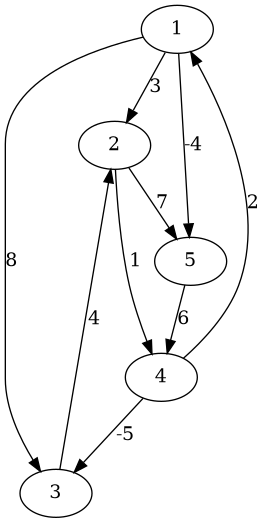
\includegraphics[scale=0.5]{images/apsp_01.png}
\end{figure}

The corresponding weight matrix has the following structure

\bee
\Wbf = \begin{pmatrix} 0 & 3 & 8 & \infty & -4 \\
  \infty & 0 & \infty & 1 & 7 \\
  \infty & 4 & 0 & \infty & \infty \\
  2 & \infty & -5 & 0 & \infty \\
  \infty & \infty & \infty & 6 & 0
\end{pmatrix}
\eee

Let's start with $l^1_{1,4} = \min_k \left(l^0_{1,k} + w_{k,4} \right)$. For different values of $k$, we obtain the following values

\begin{tabular}{c|c}
  k & $l^0_{1,k} + w_{k,4}$  \\ \hline
  1 & $0 + \infty = \infty$ \\
  2 & $3 + 1 = 4$ \\
  3 & $8 + \infty = \infty$ \\
  4 & $\infty + 0 = \infty$ \\
  5 & $-4 + 6 = 2$
\end{tabular}

The minimum, therefore, is $2$ and we have $l^1_{1,4} = 2$. Calculating the other matrix elements the same way (using \verb Extend-Shortest-Path(L,W) , yields the following for $\Lbf^2$:

\bee
\Lbf^2 = \begin{pmatrix} 0 & 3  & 8 & \infty & -4 \\
 \infty &  0 &  \infty & 1 & 7 \\
 \infty &  4 & 0 & \infty & \infty \\
    2  & \infty &  -5 & 0  & \infty \\
 \infty & \infty & \infty &  6 &  0  
  \end{pmatrix}
\eee

Executing \verb Slow-All-Pairs-Shortest-Paths(W) we finally obtain the matrix with all shortest path weights as follows

\bee
\Lbf^4 = \begin{pmatrix} 0 & 1  & -38 & 2 & -4 \\
 3 &  0 &  -4 & 1 & -1 \\
 7 &  4 & 0 & 5 & 3 \\
 2  & -1 & -5 & 0  & -2 \\
 8 & 5 & 1 &  6 &  0  
  \end{pmatrix}
\eee

Repeated application of \verb Extend-Shortest-Path(L,W) yields fewer and fewer infinite values as the algorithm finds ways / paths to connect vertices with each other. This causes the infinite path weight values to vanish. 

%%% Local Variables:
%%% mode: latex
%%% TeX-master: "journal"
%%% End:
